\documentclass{tufte-handout}

\title{CS224n: Natural Language Processing with Deep Learning
       \thanks{Course Instructors: Christopher Manning, Richard Socher} \\
       \Large Lecture Notes:  TensorFlow\thanks{Authors: Zhedi Liu, Jon Gauthier, Bharath Ramsundar, Chip Huyen}}

\date{Winter 2017} % without \date command, current date is supplied

%\geometry{showframe} % display margins for debugging page layout

\usepackage{graphicx} % allow embedded images
  \setkeys{Gin}{width=\linewidth,totalheight=\textheight,keepaspectratio}
  \graphicspath{{tensorflow/fig/}} % set of paths to search for images
\usepackage{amsmath}  % extended mathematics
\usepackage{amstext}  % extended text
\usepackage{booktabs} % book-quality tables
\usepackage{units}    % non-stacked fractions and better unit spacing
\usepackage{multicol} % multiple column layout facilities
\usepackage{lipsum}   % filler text
\usepackage{fancyvrb} % extended verbatim environments
\usepackage{placeins}
  \fvset{fontsize=\normalsize}% default font size for fancy-verbatim environments
\usepackage[normalem]{ulem}
\usepackage{algpseudocode}
\usepackage{algorithm}
\usepackage{listings}

\usepackage{sty/code_snippet}

% tikz package
\usepackage{tikz}
\usetikzlibrary{patterns, shapes,calc,positioning,arrows,mindmap,matrix}
\usetikzlibrary{decorations.pathreplacing}

% Standardize command font styles and environments
\newcommand{\doccmd}[1]{\texttt{\textbackslash#1}}% command name -- adds backslash automatically
\newcommand{\docopt}[1]{\ensuremath{\langle}\textrm{\textit{#1}}\ensuremath{\rangle}}% optional command argument
\newcommand{\docarg}[1]{\textrm{\textit{#1}}}% (required) command argument
\newcommand{\docenv}[1]{\textsf{#1}}% environment name
\newcommand{\docpkg}[1]{\texttt{#1}}% package name
\newcommand{\doccls}[1]{\texttt{#1}}% document class name
\newcommand{\docclsopt}[1]{\texttt{#1}}% document class option name
\newenvironment{docspec}{\begin{quote}\noindent}{\end{quote}}% command specification environment
\newcommand{\argmin}{\operatornamewithlimits{argmin}}
\newcommand{\argmax}{\operatornamewithlimits{argmax}}
\newcommand{\textunderscript}[1]{$_{\text{#1}}$}

\setcounter{secnumdepth}{3}
\setcounter{tocdepth}{3}


\begin{document}

\maketitle% this prints the handout title, author, and date

\textbf{Keyphrases: TensorFlow} \\
\noindent
\textbf{Code Demo: \url{https://github.com/nishithbsk/tensorflow_tutorials}}

\section{Introduction}
TensorFlow is an open source software library for numerical computation using data flow graphs. It was originally developed by researchers and engineers working on the Google Brain Team within Google's Machine Intelligence research organization for the purposes of conducting machine learning and deep neural networks research. \\

\marginnote{Check the official tutorial\\ \url{https://www.tensorflow.org/get_started/}}

Nodes in TensorFlow's data flow graph represent mathematical operations, while the edges represent the multidimensional data arrays (tensors) communicated between them. The advantage of the flexible architecture is that it allows users to build complex models step by step and makes gradient calculations simple. TensorFlow programs use a tensor data structure to represent all data -- only tensors are passed between operations in the computation graph. You can think of a TensorFlow tensor as an n-dimensional array or list. A tensor has a static type, a rank, and a shape.

\section{Concepts}
\subsection{Variables, Placeholders, Mathematical Operations}
Let's use $$h = ReLU(Wx + b)$$ where $ReLU$ (Rectified Linear Unit) is defined as $f(x) = max(0, x)$ as an example to take a closer look at TensorFlow's data flow graph, shown in Figure~\ref{fig:tensorFlow}. There are three types of nodes in a flow graph: variables, placeholders and mathematical operations.

\begin{marginfigure}
	\centering
	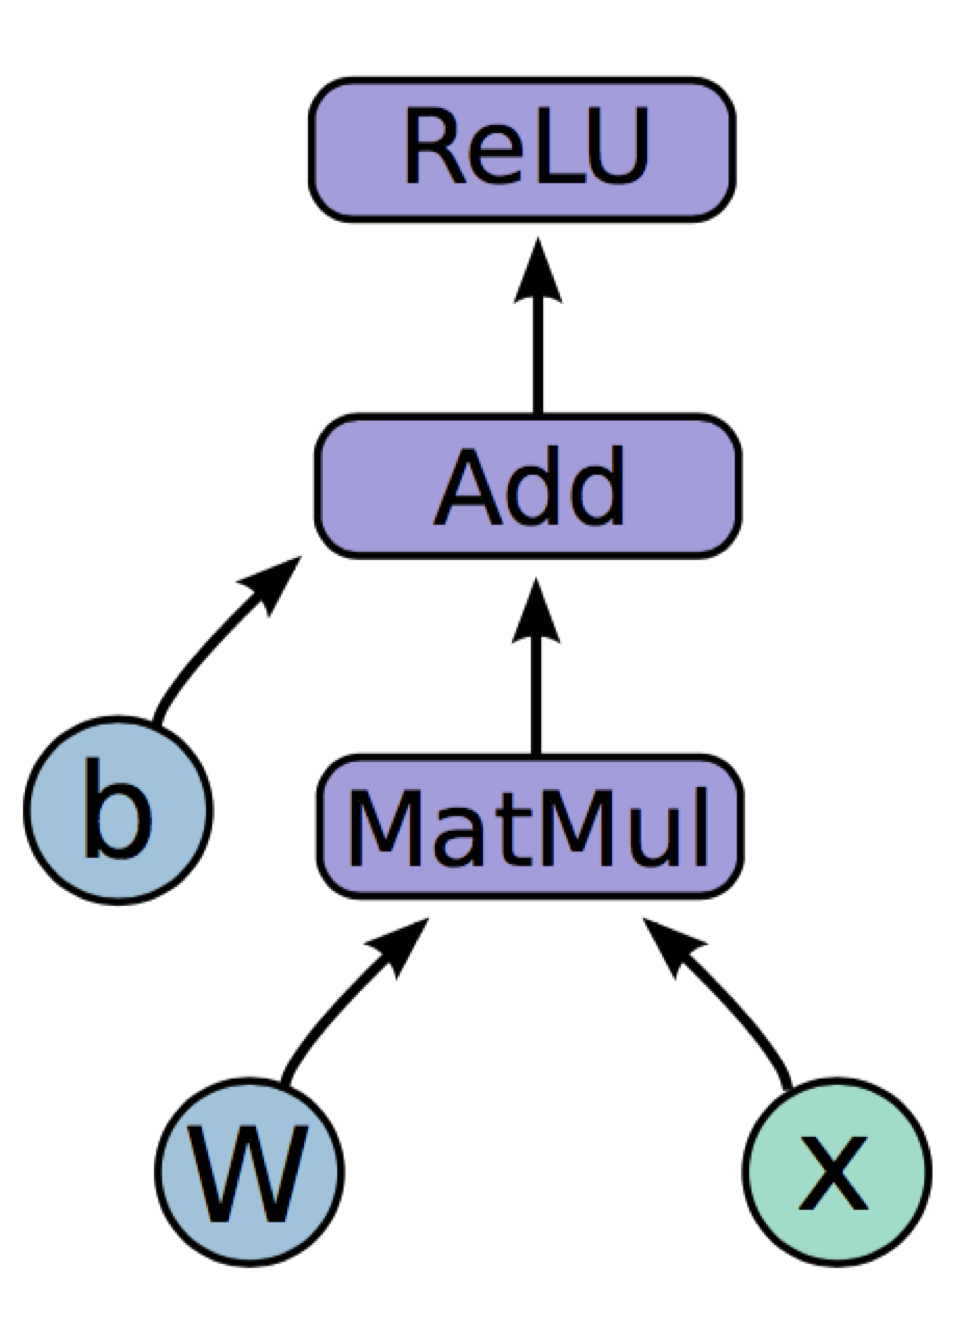
\includegraphics[width=\linewidth]{tensorFlow.png}
	\caption {An Illustration of a TensorFlow Flow Graph}
	\label{fig:tensorFlow}
\end{marginfigure}

Variables are stateful nodes that maintain state across executions of the graph. By stateful, we mean that variables retain their current values over multiple executions, and it's easy to restore those saved values. Variables can be saved to disk during and after training. Typically, variables are parameters in a neural network. In our example, weights $W$ and bias $b$ are variables.

Placeholders are nodes whose values are fed in at execution time. The rationale behind having placeholders is that we want to be able to build flow graphs without having to load external data, as we only want to pass in them at run time. Placeholders, unlike variables, require initialization. In order to initialize a placeholder, type and shape of data have to be passed in as arguments. Input data and labels are some examples that need to be initialized as placeholders. In our example, placeholder is $x$. See the code snippet below for initializing an input placeholder that has type tf.float32 and shape (batch\_size, n\_features), and a labels placeholder that has type tf.int32 and shape (batch\_size, n\_classes).


\begin{python}
## Example code snippet
input_placeholder = tf.placeholder(tf.float32,
					shape=(batch_size, n_features))
labels_placeholder = tf.placeholder(tf.int32, s
					hape=(batch_size, n_classes))
\end{python}

Mathematical operations, as the name suggests, represent mathematical operations in a flow graph. In our example, \texttt{MatMul} (multiply two matrix values), \texttt{Add} (add element-wise with broadcasting) and \texttt{ReLU} (activate with element-wise rectified linear function) are mathematical operations.

Now we are ready to see our flow graph in code. Let's assume our input $x$ has shape ($N$, $Dx$), $W$ has shape ($Dx$, $N$) and type tf.float32, $b$ has shape ($N$, 1) and we will initialize $W\sim \textrm{Uniform}(-1, 1)$ and $b = \boldmath{0}$. Then the code snippet below shows us how to build our flow graph for $h = ReLU(Wx + b)$.

\begin{python}
## Example code snippet
import tensorflow as tf

b = tf.Variable(tf.zeros((N,)))
W = tf.Variable(tf.random_uniform((Dx, N), -1, 1))
x = tf.placeholder(tf.float32, (N, Dx))
h = tf.nn.relu(tf.matmul(x, W) + b)

\end{python}

The key thing to remember about symbolic programming language is that, up to what what we have written here, no data is actually being computed. $x$ is just a placeholder for our input data. A flow graph merely defines a function. We cannot do \texttt{print(h)} and gets its value as it only represents a node in the graph.

\subsection{Fetch, Fetch}
Now that we've defined a graph, the next steps are to deploy this graph with a session and run the session to get our outputs. A session is an environment that supports the execution of all operations to a particular execution context (e.g. CPU, GPU). A session can be easily built by doing \texttt{sess = tf.Session()}. In order for a session to run, two arguments have to be fed: fetches and feeds. We use feeds and fetches to get data into and out of arbitrary operations.

Fetches represent a list of graph nodes and return the outputs of these nodes. We could fetch a single node or multiple tensors. See the code snippet below for an example of fetching two tensors: \texttt{mul} and \texttt{intermed}.

\begin{python}
## Example code snippet
import tensorflow as tf

input1 = tf.constant([3.0])
input2 = tf.constant([2.0])
input3 = tf.constant([5.0])
intermed = tf.add(input2, input3)
mul = tf.mul(input1, intermed)

with tf.Session() as sess:
  result = sess.run([mul, intermed])
  print(result)

# output:
# [array([ 21.], dtype=float32), array([ 7.], dtype=float32)]

\end{python}

A feed, supplied as an argument to a \texttt{run()} call, temporarily replaces the output of an operation with a tensor value. The feed is only used for the \texttt{run} call to which it is passed. Essentially, feeds are dictionaries mapping placeholders to their values. Nodes that depend on placeholders cannot run unless their values are fed. See the code snippet below for an example of feeding a \texttt{feed\_dict}.

\begin{python}
## Example code snippet
import tensorflow as tf

input1 = tf.placeholder(tf.float32)
input2 = tf.placeholder(tf.float32)
output = tf.mul(input1, input2)

with tf.Session() as sess:
  print(sess.run([output], feed_dict={input1:[7.], input2:[2.]}))

# output:
# [array([ 14.], dtype=float32)]

\end{python}

Before moving on to how to train a model, let's see a slightly more complicated example combining fetch and feed. In this example, we have a placeholder $x$ that requires initialization. We have two variables $W$ and $b$. It should be noted that when we launch a graph, all variables have to be explicitly initialized before one can run Ops that use their value. A variable can be initialized by running its initializer op, restoring the variable from a save file, or simply running an assign Op that assigns a value to the variable. In fact, the variable initializer op is just an assign Op that assigns the variable's initial value to the variable itself. An example usage is \texttt{sess.run(w.initializer)} where $w$ is a variable in the graph. The more common initialization pattern is to use the convenience function \texttt{tf.initialize\_all\_variables()} to add an Op to the graph that initializes all the variables, as illustrated in the code snippet below.

\begin{python}
## Example code snippet
import numpy as np
import tensorflow as tf

b = tf.Variable(tf.zeros((100,)))
W = tf.Variable(tf.random_uniform((784, 100),
                -1, 1))

x = tf.placeholder(tf.float32, (100, 784))
h = tf.nn.relu(tf.matmul(x, W) + b)

sess = tf.Session()
sess.run(tf.initialize_all_variables())
# {x: np.random.random(100, 784)} is a feed
# that assigns np.random.random(100, 784) to placeholder x
sess.run(h, {x: np.random.random(100, 784)})

\end{python}

\subsection{How to Train a Model in TensorFlow}

\textit{1. Define a Loss} \\
The first thing to do in order to train a model is to build a loss node. See the code snippet below for an example of defining a cross-entropy loss. We build the loss node using labels and prediction. Note that we use \texttt{tf.reduce\_sum} to compute the sum of elements across dimensions of a tensor. For our example, \texttt{axis=1} is used to perform a row-wise sum.

\begin{python}
## Example code snippet
import tensorflow as tf

prediction = tf.nn.softmax(...)  #Output of neural network
label = tf.placeholder(tf.float32, [100, 10])

cross_entropy = -tf.reduce_sum(label * tf.log(prediction), axis=1)

# More examples of using tf.reduce_sum
# 'x' is [[1, 1, 1]
#         [1, 1, 1]]
# tf.reduce_sum(x) ==> 6
# tf.reduce_sum(x, 0) ==> [2, 2, 2]
# tf.reduce_sum(x, 1) ==> [3, 3]
# tf.reduce_sum(x, 1, keep_dims=True) ==> [[3], [3]]
# tf.reduce_sum(x, [0, 1]) ==> 6
\end{python}

\noindent
\textit{2. Compute Gradients} \\
The next thing we have to do is to compute gradients. TensorFlow nodes have attached operations; therefore gradients with respect to parameters are automatically computed with backpropagation. All we need to do is creating an optimizer object and calling the \texttt{minimize} function on previously defined loss. See code snippet below for an example of using a \texttt{GradientDescentOptimizer} optimizer where \texttt{cross\_entropy} is the same as we introduced in the previous code snippet. Evaluating the minimization operation, \texttt{train\_step} at runtime will automatically compute and apply gradients to all variables in the graph.

\begin{python}
## Example code snippet
import tensorflow as tf

lr = 0.5 # learning rate
optimizer = tf.train.GradientDescentOptimizer(lr)
train_step = optimizer.minimize(cross_entropy)
\end{python}

\noindent
\textit{3. Train Model} \\
Now we are ready to train a model. This can simply be done by creating an iterating training schedule that feeds in data, labels and applies gradients to the variables, as shown in the code snippet below.

\begin{python}
## Example code snippet
import tensorflow as tf

sess = tf.Session()
sess.run(tf.initialize_all_variables())

for i in range(1000):
	batch_x, batch_label = data.next_batch()
	sess.run(train_step, feed_dict={x: batch_x, label: batch_label}
\end{python}

\subsection{Variable Sharing}
One last important concept is variable sharing. When building complex models, we often need to share large sets of variables and might want to initialize all of them in one place. This can be done by using \texttt{tf.variable\_scope()} and \texttt{tf.get\_variable()}.

Imagine we are building a neural nets with two layers, if we use \texttt{tf.Variable}, we would have two sets of weights and two sets of biases. Let's assume that these variables are initialized in \texttt{define\_variables()}. The problem arises when we want to use this model for two tasks that share the same parameters. We would have to call \texttt{define\_variables(inputs)} twice, resulting in two sets of variables, 4 variables in each one, for a total of 8 variables. A common try to share variables is to create them in a separate piece of code and pass them to functions that use them, say by using a dictionary. I.e. the \texttt{define\_variables} now takes two arguments, \texttt{inputs} and \texttt{variables\_dict}. While convenient, creating a \texttt{variables\_dict}, outside of the code, breaks encapsulation: 1) the code that builds the graph must document the names, types, and shapes of variables to create, and 2) When the code changes, the callers may have to create more, or less, or different variables. One way to address the problem is to use classes to create a model, where the classes take care of managing the variables they need. For a lighter solution, not involving classes, TensorFlow provides a Variable Scope mechanism that allows to easily share named variables while constructing a graph.

Variable Scope mechanism in TensorFlow consists of two main functions: \texttt{tf.get\_variable(<name>, <shape>, <initializer>)} creates or returns a variable with a given name instead of a direct call to \texttt{tf.Variable}; \texttt{tf.variable\_scope(<scope\_name>)} manages namespaces for names passed to \texttt{tf.get\_variable()}. \texttt{tf.get\_variable} does one of two things depending on the scope it is called in. Let's set \texttt{v = tf.get\_variable(name, shape, dtype, initializer)}.

Case 1: the scope is set for creating new variables, i.e. \texttt{tf.get\_variable\_scope(name, reuse=False)}.In this case, $v$ will be a newly created \texttt{tf.Variable} with the provided shape and data type. The full name of the created variable will be set to the current variable scope name + the provided name and a check will be performed to ensure that no variable with this full name exists yet. If a variable with this full name already exists, the function will raise a \texttt{ValueError}. If a new variable is created, it will be initialized to the value \texttt{initializer(shape)}. For example,

\begin{python}
## Example code snippet
import tensorflow as tf

with tf.variable_scope("foo"):
    v = tf.get_variable("v", [1])
assert v.name == "foo/v:0"
\end{python}

Case 2: the scope is set for reusing variables, i.e. \texttt{tf.get\_variable\_scope(name, reuse=True)}. In this case, the call will search for an already existing variable with name equal to the current variable scope name + the provided name. If no such variable exists, a \texttt{ValueError} will be raised. If the variable is found, it will be returned. If a variable already exists but \texttt{reuse=False}, program will crash. For example:

\begin{python}
## Example code snippet
import tensorflow as tf

with tf.variable_scope("foo"):
    v = tf.get_variable("v", [1])
with tf.variable_scope("foo", reuse=True):
    v1 = tf.get_variable("v", [1])
with tf.variable_scope("foo", reuse=False):
	v1 = tf.get_variable("v") 	   # CRASH foo/v:0 already exists!
\end{python}



\end{document}
